\chapter{Apparatus}

%%
%% CONSIDERATIONS
%%
\section{Background}
These experiments require a fixture that will repeatably hold the three key components of the experiment set-up: the battery cell being tested, the transmitting transducer, and the receiving transducer. 
There are a number of positional requirements. 
If the transducers are not axially-aligned, nontrivial errors can be introduced to the time of flight measurements.
If all surfaces between the two transducer faces do not align squarely, the waves will travel through air, introducing error to the time of flight measurements. 
The apparatus is also limited in where it may contact the cell. It has to leave the edges clear, because the lamination sealing the cell's outer layer sometimes causes small bulges, which could prevent the apparatus from pressing rigidly against both sides of the cell.

The apparatus would need to be able to apply a consistent and controllable pressure to the battery cell. 
This is due to the emerging role of stack pressure in the state of health of a cell. 
Canarella showed that, when a cell is held such that it cannot expand, stack pressure builds up as it cycles, causing chemical degradation to the electrode and potentially inhibiting transport \cite{STACK-STRESS}. Stack stress has a material effect on battery state of health and must be controlled for.
\todo{cite}
Thus, the apparatus must hold the cell rigidly enough to prevent gaps forming in the acoustic pathway from the transmitting transducer to the receiving transducer, yet must also not apply so much pressure that it inhibits the very behavior which the experiment is intended to observe. 
The pressure should be adjustable. This is in part because cells of different geometries will require different forces to experience a particular stack pressure. 
Additionally, Cannarella defined low, medium, and high stack pressure regimes, and the high pressure regime could be used to induce lithium plating if need be \cite{STACK-STRESS}.

After initial experimentation, it became clear that the apparatus would also have to be relatively temperature controlled. 
Temperature fluctuations lead to material changes in time of flight through the cell, introducing so much noise to the data that the signal was totally obscured.
A thermal chamber was added to the set-up to hold the temperature of the cell and transducers more constant, along with thermocouples and a microcontroller to log the temperature data for use during the electrochemical-acoustical analysis.

\section{Transducer Considerations}
\subsection{Frequency versus Attenuation}
The transducers introduce a number of important considerations into the design process.
The selected transducers were 15 MHz. The fast-charge cells are quite thin, and lithium plating on their electrode would have a thickness on the order of microns. 
For such a small change in thickness to be perceptible by the transducers, they would need to have a very small wavelength \todo{why}. Due to the simple relationship 
$$ \lambda = c/f$$
a transducer with a small wavelength will have an accordingly large frequency. At such a high frequency, the readings will be quite susceptible to attenuation, which increases linearly with the square of frequency and the square of bandwidth \cite{OLYMPUS}, putting resolution and attenuation at odds. Attenuation is \todo{what is}.

\subsection{Near-Field Effects}
The sound field of a transducer is not constant, but rather split into two zones with distinct behavior: the near-field (or Fresnel) zone, and the far-field (or Fraunhofer) zone \cite{OLYMPUS}. 
The near-field zone is a small region immediately following the transducer, and is a place of considerable noise due to rapid switches between energy minima and maxima. 
The last of these maxima is located at the near field distance $N$, and forms the boundary between the near field and far field regions. \cite{OLYMPUS}
In the far-field, sound field pressure decreases monotonically and gently until it reaches zero. \cite{OLYMPUS}
It is a much more predictable zone and thus more suited to the delicate amplitude measurements required for accurate time of flight measurements at this scale.
The apparatus should position the transducers relative to the battery cell such that it falls into the far field region, but not so far into that region that the sound field pressure has become unworkably weak.

\subsection{Impedance}
Acoustic impedance is a material's "opposition to displacement of its particles by sound" \cite{OLYMPUS}. It must be minimized in the path between the transducer and the cell in order ensure strong readings. Acoustic impedance, $Z$, is a function of
$$ Z = \rho c$$
where $\rho$ is the material's density and $c$ is the material's sound velocity \cite{OLYMPUS}.
At the boundary between two materials - the acoustic interface - impedance differences cause energy losses. At an acoustic boundary, part of a wave is transmitted, and part reflected; each signal experiences energy loss due to the acoustic interface, but the magnitude varies depending on the relative magnitudes of the two material's impedances.
For the transmitted wave, the loss can be calculated as follows:
$$ \text{dB loss} = 10 \log_{10} \frac{4Z_1 Z_2}{(Z_1 + Z_2)^2}$$
where $Z_1$ is the impedance of the first material and $Z_2$ is the impedance of the second \cite{OLYMPUS}.

For the reflected wave, 
$$\text{dB loss} = 10\log_{10} \frac{(Z_2 - Z_1)^2}{(Z_1 + Z_2)^2} \cite{OLYMPUS}$$

For reflected waves, it is clear that the relative magnitude of the two impedances is very important, with materials of more similar impedances causing less loss.

%%
%% STRUCTURE %%
%%
\section{Structure}
\todo{PIC cad ass whole}

The basic apparatus is a pair of blocks mounted to a rail. A row of holes is drilled into the blocks to hold an array of ultrasonic transducers, with channels milled out for routing their cables. A small plate with its own set of holes and channels bolts to this block to hold the transducers in place. Bolting to this plate is a small cylinder of Rexolite (a nylon variant), used as a low-interference medium for manipulating the travel distance of the ultrasonic waves to eliminate near-field effects, as will be discussed in greater detail later.

\todo{PIC cad part block}
Behind the first set of holes in the block is a second set of narrower holes, for spring-loading the transducers. The springs ensure the transducers are pressed against the face of the transfer medium. The faces of the Rexolite cylinders are turned flat so that the transducer emits and receives waves at an angle perpendicular to the test article. \todo{PIC cad part plate} The plate further facilitates keeping everything coaxial. The three parts bolt together using one set of bolts which pass through all three, ensuring a tight, flat fit \todo{PIC subass block plate Rexolite ducers bolts}. This both keeps the transducers perpendicular to the test article and coaxial with each each other, as well as preventing any disruptive air from getting in the path of the ultrasonic waves, allowing unnecessary attenuation to reduce the quality of the data. 

\subsection{Manufacturing Considerations}
Aluminum was chosen as the material for the blocks for its durability and machinability. Machinability was important because of the relatively tight tolerances required of these parts. Since the test articles are so thin and the ultrasonic transducers to high-frequency, small differences in actual versus expected transducer position could create insurmountable noise in the readings. Of particular importance were flatness of the various components (so that small angles are not introduced to the transducer position) and accuracy of the hole positions for the transducers relative to each other and to the mounting hole for the piston rod. Additionally, the fit of the holes for the transducers is important; it must be snug enough that they transducers are held perpendicular to the test article and not allowed to rock around, while also allowing free enough translational movement along their center axis for the springs to be able to push them firmly against the transmission medium.

The total apparatus has two of these block assemblies. One block is bolted directly to the rail and held stationary during the tests. The other is connected to via threaded rod to a double-acting piston and fixed to a carriage which rides along the rail. The piston is fixed to the rail by a bracket, and extends to push the block along the rail, securing the cell. By varying the pressure supplied to the piston, it can be used to apply a controlled stack pressure to the cell during testing.

\subsection{Transmission Media}
The Rexolite cylinder is included in the assembly as a transmission medium to ensure that the ultrasonic waves traverse the cell during Fraunhofer (far field) diffraction, rather than during noisy Fresnel (near field) diffraction. The extent of the near field $N$ is determined as follows:
$$\label{eq:nearfield} N= \frac{D^2 f} {4c} $$
where $D$ is the element diameter, $f$ is the wave frequency, and $c$ is the material sound velocity \cite{OLYMPUS}.
\begin{figure}[t]\label{fig:fieldEffects}
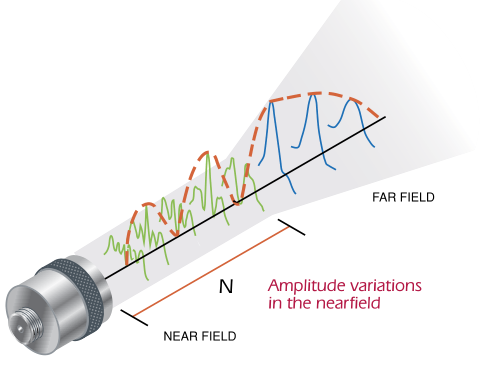
\includegraphics[]{fields-olympus-45}
\centering
\caption{An illustration of Fresnel and Fraunhofer fields from \cite{OLYMPUS}}
\end{figure}
$f$ needs to be kept high for this experiment, because thinner cells require shorter wavelengths and thus greater frequencies to generate data at a useful resolution, and the cells of interest have a thickness on the order of microns. $D$ is fixed characteristic of the sensors. $c$ is a function of the transmission medium, and a medium besides the case of the cell will be necessary if $N$ is greater than the cell casing thickness, which in this case it is. The only one of those variables which is able to be somewhat manipulated for this experiment is $c$, which is an important consideration in transmission media materials selection. 
Thus, to avoid near field effects, the transducers must be mounted far enough from the cell that the wave does not enter the cell until after it has entered the far field regime. The near-field distance for combinations of two different transducers and two different transmission media is shown in \autoref{tab:nearfield}. The table shows that 1) ultrasonic transducers create waves which have much too large a near field to be mounted directly against the cell under test, and 2) in order for the apparatus to be useful with more ultrasonic sensors operating at different frequencies, the transmission media for the apparatus need to be modular so as to swap in transmission media of different sizes. In theory one could also change the material of the media to counteract greater or smaller near field effects, but it is more practical to change the size of the component. 

\begin{table}[h]
    \centering
    \begin{tabular}{c|c|c|c}
         $f$ (MHz) & $D$ (mm) & $c$ (m/s) & $N$ (cm) \\
         \hline
         10 & 6.35 & 2400 & 4.2 \\
         20 & 6.35 & 2400 & 8.4 \\
         10 & 6.35 & 2600 & 3.88 \\
         20 & 6.35 & 2600 & 7.75 \\
    \end{tabular}
    \caption{Near-field distance $N$ as a function of frequency $f$, element diameter $D$, and material sound velocity $c$.}
    \label{tab:nearfield}
\end{table}


Introducing a distance between the transducers and cell allows the analysis to avoid accommodating Fresnel diffraction, but also introduces some losses due to the acoustic interface at the change in transmission media. The magnitude of the losses depends in part on the difference in the impedances of the two media, so Rexolite (a variety of Nylon) was selected for its similar impedance to the aluminized polymer that comprises the outer layer of the battery cell, keeping the signal attenuation to a minimum.
The decibel loss of energy due to an acoustic interface is 
$$\text{dB loss} = 10\log _{10} \frac{(Z_2 - Z_1)^2}{(Z_1 + Z_2)^2}$$
where $Z_1$ is the impedance of the material being transmitted out of, and $Z_2$ is the impedance of the material being transmitted into \cite{OLYMPUS}. This can easily be transformed into the percentage of energy transmitted across an acoustic interface:
$$ \frac{E_{transmitted}}{E_{total}} = 1 - \bigg{(}\frac{Z_2 - Z_1}{Z_1 + Z_2} \bigg{)}^2$$

For the acoustic interface between the Rexolite and the outer polyamide film on the cell, with $Z_1 = 2.5$ \cite{REXOLITE} and $Z_2 = 3.1$ \cite{OLYMPUS}, 98.9\% of the energy is transmitted across the acoustic interface. Since there is a spacer both between the cell and the transmitting transducer and between the cell and the receiving transducer, the transmitted energy is actually $98.9*98.9 = 97.7\%$ of the sent energy, not including transmission losses due to acoustic interfaces within the cell or due to other causes. For the interface coming out the back of the cell and into the other spacer,  Therefore, Rexolite makes an excellent material to serve as the acoustic spacer between the transducer and the cell. 

Additionally, Rexolite takes to machining and finishing well, and for this material, it was important to be able to machine a flat surface onto the faces which contact the ultrasonic transducers and the test articles, in order to keep any dust or air from getting into the path of the ultrasonic waves and introducing noise to the readings.
 
%%
%% ACTUATOR
%%
\section{Actuator}
The pneumatic piston was chosen as the actuator primarily for its relatively high precision and its relatively low cost. Other advantages include the relatively low set-up and calibration time required, its ease of control by adding an electronic or manually set pressure regulator into its air line, and its lack of any extraneous degrees of freedom. This piston in particular was chosen for having an internal double rail, which further reduces the potential for the piston to introduce misalignment into the system. Another factor considered in choosing the particular piston were its form factor. The chosen piston has flat sides and copious mounting holes, making it convenient to mount into the apparatus. Another important consideration is range of pressure outputs. While most of the time the desired stack pressure will likely be in Cannarella's "low" stack pressure regime (0-0.5MPa) \cite{STACK-STRESS}, it is useful to leave open the option of inducing Cannarella's "high" stack pressure regime \cite{STACK-STRESS}, peaking at as much as 3.0 MPa, in order to intentionally induce lithium plating, if necessary.
Stack pressure $P_{stack}$ applied by the actuator as a function of the actuator's gauge pressure $P_{gauge}$ and nominal force output $F$ at pressure $P_{nom}$ was calculated as follows:
$$P_{stack} = F_{P_{nom}}\frac{P_{gauge}}{P_{nom}}\frac{1}{A} $$
This calculation determined that the following forces would be required of the actuator to implement each of Cannarella's regimes:

\begin{table}[h]
    \centering
    \begin{tabular}{c|c|c|c}
         Regime & $P_{Stack}$ (MPa) & Applied Force (kN) & $P_{gauge}$ (MPa) \\
         \hline
         low & 0-0.5 & 0 - 1 & 0 - 0.03 \\
         medium & 0.2-1.5 & 0.4 - 3 & 0.01 - 0.09 \\
         high & 1-3 & 2 - 6 & 0.06 - 0.17 \\
    \end{tabular}
    \caption{Actuator parameters necessary for each of Cannarella's stack pressure regimes.}
    \label{tab:stackpressure}
\end{table}

Thus, it is useful to have a piston capable of a broad range of output forces. A final useful feature is the piston's double acting configuration, which allows the piston to instantaneously either extend or retract without needing to reroute airlines. The piston is actuated by a relay and controlled by a Particle Photon microcontroller.

%%
% THERMAL CHAMBER
%%
\section{Thermal Chamber}\label{thermalChamber}
A modified minifridge serves as a thermal chamber to hold the temperature roughly constant during the tests. 
Some of the fridge's insulation needed to be cut away to allow airlines for the actuator to pass out of the fridge to the air source so it does not perfectly hold temperature, but the results are constant enough that a validation test confirmed that the thermal chamber prevents temperature-induced noise from overwhelming the acoustic signal; see \hyperref[chamberTest]{\cref{chamberTest}}.  
The thermal chamber's temperature is not actively controlled; rather, it passively maintains its internal temperature by means of well-insulated walls and high thermal inertia filler (water-filled plastic containers). 
Its temperature is monitored by three thermocouples.

\section{Electronics}

\todo{flowchart}

Signal is created by a signal generator, per programmed parameters. This is passed through the transducer, which forms it into an acoustic wave. It passes this wave through the test unit to be received by a second transducer opposite it on the other side of the unit. The reading transducer is connected to a signal scope (the Picoscope unit) which reads this signal and reports it to the computer.

Simultaneously, the Neware cycler unit is using a standard four-lead set-up to both induce a load on the cell and to monitor the cell's state. The cycler sends a signal through the leads of the cell via one pair of leads, and uses a second pair of leads to read the cell's current and voltage. Timestamps connect this electrochemical data to the acoustic data.

A trio of thermocouples monitors the temperature within the thermal chamber, to ensure that time of flight shifts are due to changes in the cell's state rather than its temperature. These are read across a simple voltage divider and monitored by a microcontroller, with timestamps connecting this thermal data to the electrochemical and acoustic data.

A separate microcontroller drives the piston which applies a relatively consistent force to the cell during testing, controlling its stack pressure. A relieving pressure gauge holds the magnitude of this force to a roughly constant value, but it does not report the value and so the stack pressure is not logged. Adding this capability was considered, but it would have added expense and early trials showed that the current setup was sufficient.